\documentclass{standalone}
\usepackage{pgfplots}
\pgfplotsset{compat=newest}

\begin{document}
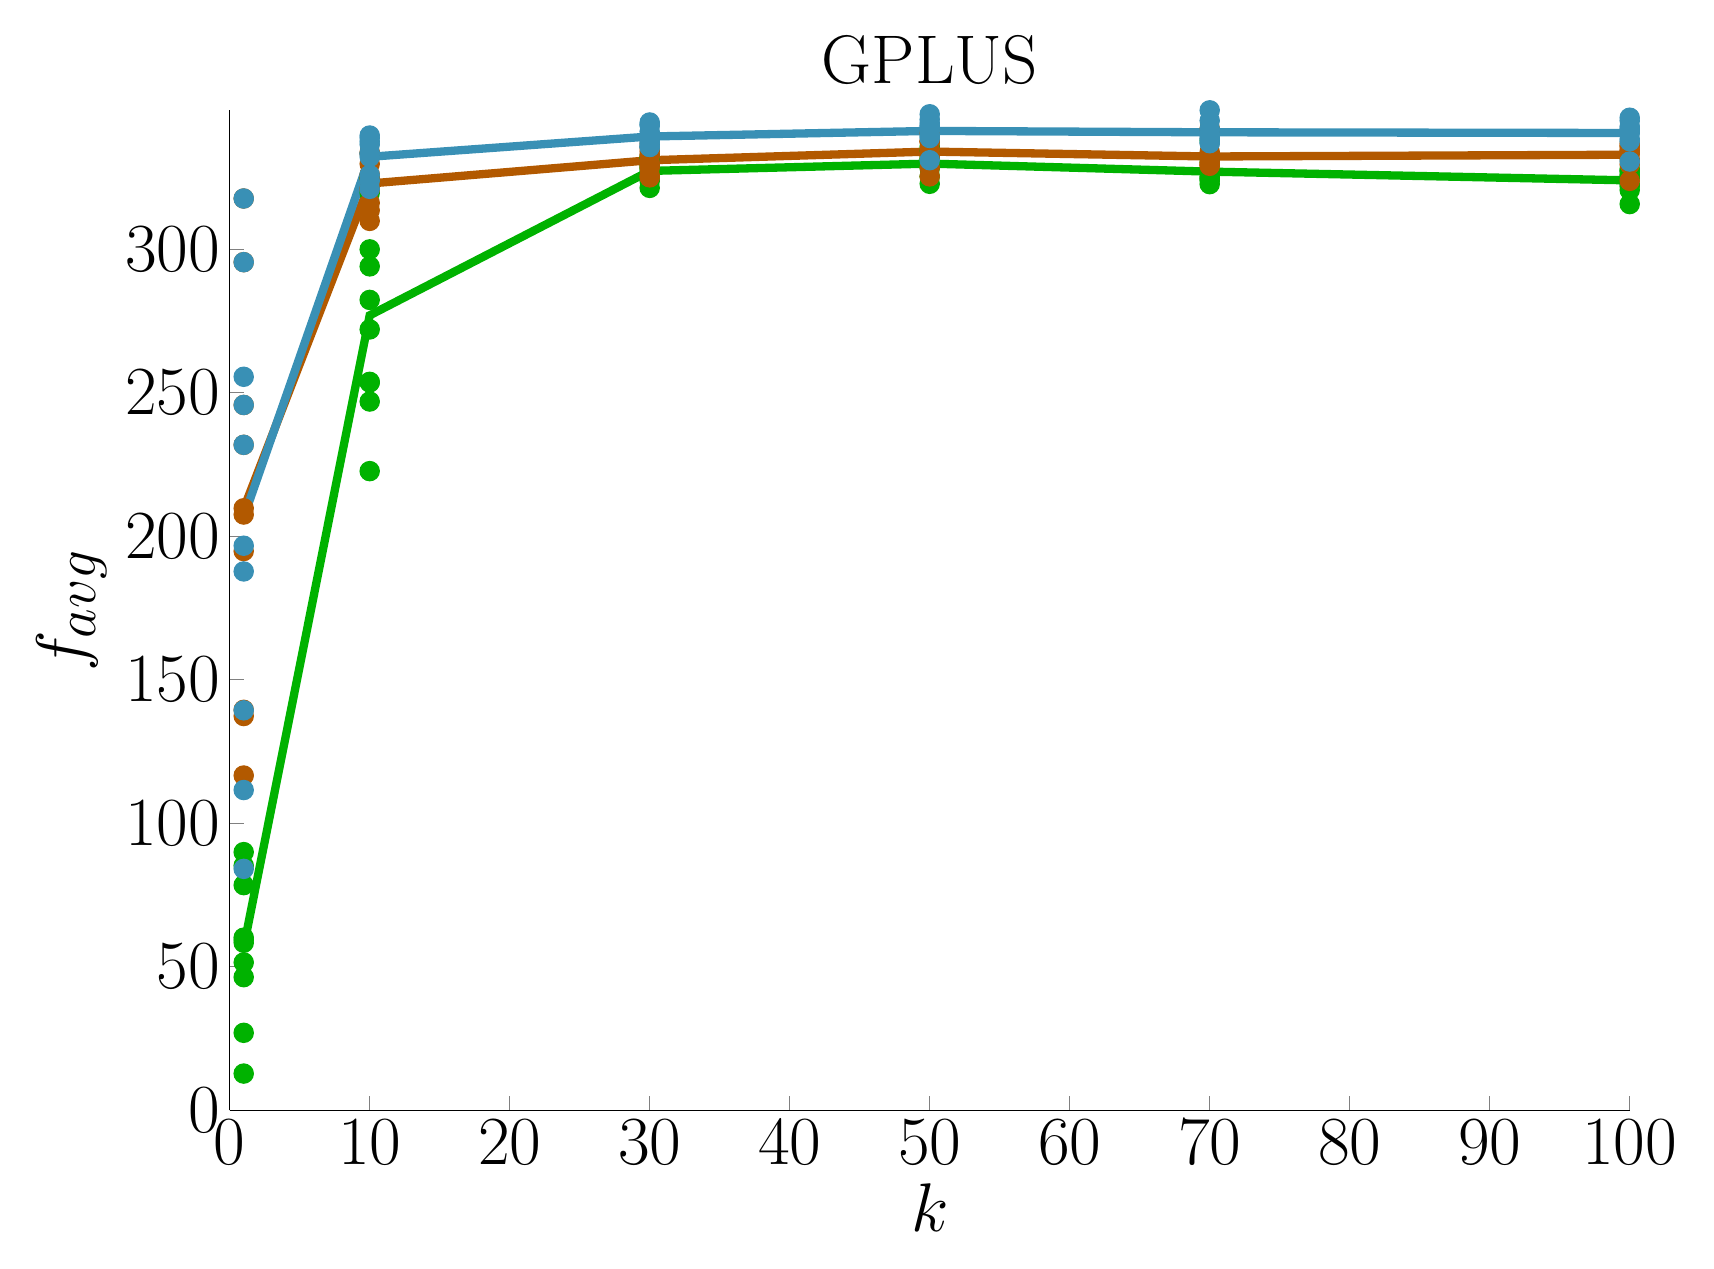
\begin{tikzpicture}

\begin{axis}[%
title style={font=\Huge},
title=GPLUS,
tick label style={font=\Huge},
label style={font=\Huge},
legend style={font=\Huge},
view={0}{90},
max space between ticks=50pt,
width=7in,
height=5in,
scale only axis,
xmin=0, xmax=100,
%xtick={0, 20, 40, 60, 80, 100},
xlabel={$k$},
ymin=0, ymax=348.32,
ylabel={$f_{avg}$},
major tick length=5pt,
axis lines*=left,
legend cell align=left,
clip=false]

\addplot [
only marks,
mark=*,
mark size=3.5pt,
color=green!70!black,
%solid,
%line width=2pt,
]
coordinates{
(1,12.8)(1,27.0)(1,46.38)(1,51.5)(1,58.36)(1,59.34)(1,60.14)(1,78.44)(1,85.24)(1,89.94)(10,222.64)(10,246.88)(10,253.52)(10,253.74)(10,272.0)(10,282.28)(10,293.96)(10,299.88)(10,319.56)(10,324.58)(30,321.3)(30,323.64)(30,324.8)(30,325.58)(30,327.14)(30,327.92)(30,328.42)(30,329.12)(30,331.88)(30,332.24)(50,322.72)(50,325.3)(50,328.12)(50,329.1)(50,329.42)(50,329.98)(50,331.38)(50,331.5)(50,334.34)(50,335.7)(70,322.6)(70,323.76)(70,324.4)(70,324.76)(70,325.22)(70,326.66)(70,326.94)(70,327.28)(70,330.3)(70,337.7)(100,315.66)(100,320.52)(100,321.88)(100,322.6)(100,324.62)(100,325.74)(100,325.82)(100,327.04)(100,327.32)(100,327.92)
};

\addplot [
only marks,
mark=*,
mark size=3.5pt,
color=orange!70!black,
%solid,
%line width=2pt,
]
coordinates{
(1,116.62)(1,137.34)(1,139.5)(1,194.8)(1,207.52)(1,209.7)(1,231.8)(1,245.68)(1,295.42)(1,317.6)(10,309.8)(10,313.48)(10,316.08)(10,320.92)(10,321.06)(10,324.48)(10,325.92)(10,329.66)(10,333.14)(10,333.68)(30,324.96)(30,325.54)(30,328.34)(30,329.5)(30,329.6)(30,332.3)(30,332.88)(30,334.1)(30,335.36)(30,336.64)(50,325.3)(50,328.42)(50,332.3)(50,332.88)(50,333.16)(50,334.74)(50,337.42)(50,337.48)(50,337.52)(50,340.28)(70,328.98)(70,329.3)(70,329.3)(70,330.18)(70,331.68)(70,332.08)(70,332.22)(70,332.78)(70,333.82)(70,342.0)(100,323.74)(100,329.48)(100,331.28)(100,333.22)(100,333.52)(100,334.28)(100,334.46)(100,335.68)(100,336.0)(100,336.84)
};

\addplot [
only marks,
mark=*,
mark size=3.5pt,
color=cyan!70!black,
%solid,
%line width=2pt,
]
coordinates{
(1,84.1)(1,111.56)(1,139.32)(1,187.7)(1,196.66)(1,231.8)(1,245.68)(1,255.5)(1,295.42)(1,317.6)(10,320.96)(10,323.8)(10,325.82)(10,332.06)(10,333.18)(10,333.34)(10,336.42)(10,337.46)(10,338.72)(10,339.54)(30,335.56)(30,335.58)(30,335.86)(30,336.9)(30,337.68)(30,339.1)(30,340.88)(30,343.02)(30,343.32)(30,344.08)(50,330.94)(50,338.66)(50,339.1)(50,339.92)(50,341.14)(50,342.68)(50,342.92)(50,343.92)(50,345.16)(50,346.94)(70,336.86)(70,337.02)(70,338.34)(70,338.6)(70,339.74)(70,339.8)(70,341.62)(70,341.62)(70,344.72)(70,348.32)(100,330.48)(100,337.56)(100,338.32)(100,340.32)(100,341.04)(100,341.44)(100,341.94)(100,342.72)(100,344.64)(100,345.74)
};
p
\addplot [
color=green!70!black,
solid,
line width=3pt
]
coordinates{
(1,56.914)(10,276.904)(30,327.204)(50,329.756)(70,326.962)(100,323.912)
};

\addplot [
color=orange!70!black,
solid,
line width=3pt
]
coordinates{
(1,209.598)(10,322.822)(30,330.922)(50,333.95)(70,332.234)(100,332.85)
};

\addplot [
color=cyan!70!black,
solid,
line width=3pt
]
coordinates{
(1,206.534)(10,332.13)(30,339.198)(50,341.138)(70,340.664)(100,340.42)
};


\end{axis}
\end{tikzpicture}
\end{document}
